% http://tex.stackexchange.com/questions/11866/compile-a-latex-document-into-a-png-image-thats-as-short-as-possible#11880
%http://tex.stackexchange.com/questions/152247/best-practice-to-include-standalone-precompiled-graphics
\documentclass[border=1pt]{standalone}
\usepackage{tikz}

\begin{document}

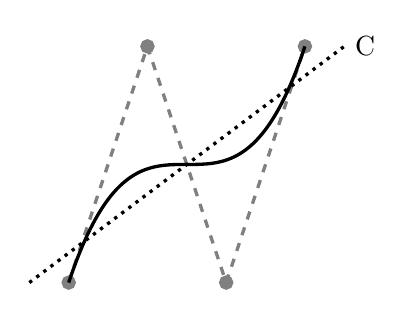
\begin{tikzpicture}[very thick]
	\coordinate (q1) at (0,0); \coordinate (q2) at (1,3);
	\coordinate (q3) at (2,0); \coordinate (q4) at (3,3);
	\draw[dashed, gray] (q1) -- (q2) -- (q3) -- (q4);
	\foreach \x in {q1,q2,q3,q4}
	{
		\draw[fill=white, gray] (\x) circle [radius=2pt];
	}
	\draw (q1) .. controls (q2) and (q3) .. (q4);
	\draw[dotted] (-0.5,0) -- (3.5,3) node[right] {C};
\end{tikzpicture}

\end{document}
